\documentclass[12pt,letterpaper]{article}

\usepackage{graphicx}
\usepackage{amssymb}
\usepackage{epstopdf}
\usepackage{multirow}
\usepackage{subfigure}
\usepackage{color}
\usepackage{hyperref}
\hypersetup{colorlinks=true,citecolor=blue}
%\usepackage{cleveref}
% ------ package for tracking changes --------% 
\usepackage[]{changes}

% -----------------------------------------------------% 

%\DeclareGraphicsRule{.tif}{png}{.png}{`convert #1 `dirname
%  #1`/`basename #1 .tif`.png}





% -----------------------------------------------------% 

\begin{document}

\title{BAND: Detector Operations Manual}



\author{
Florian Hauenstein  }
\date{\today}  

\maketitle
\begin{abstract}
This document describes the Backward Angle Neutron Detector (BAND) installed in front of the target of CLAS12, its operating procedures and the monitoring procedures to ensure the correct functioning of the detector.

\end{abstract}
\tableofcontents
%\thispagestyle{empty}
\setcounter{page}{1}
%\newpage

\section{Description of the Detector}
\subsection{Overview}
\begin{figure}[thb]
\centering
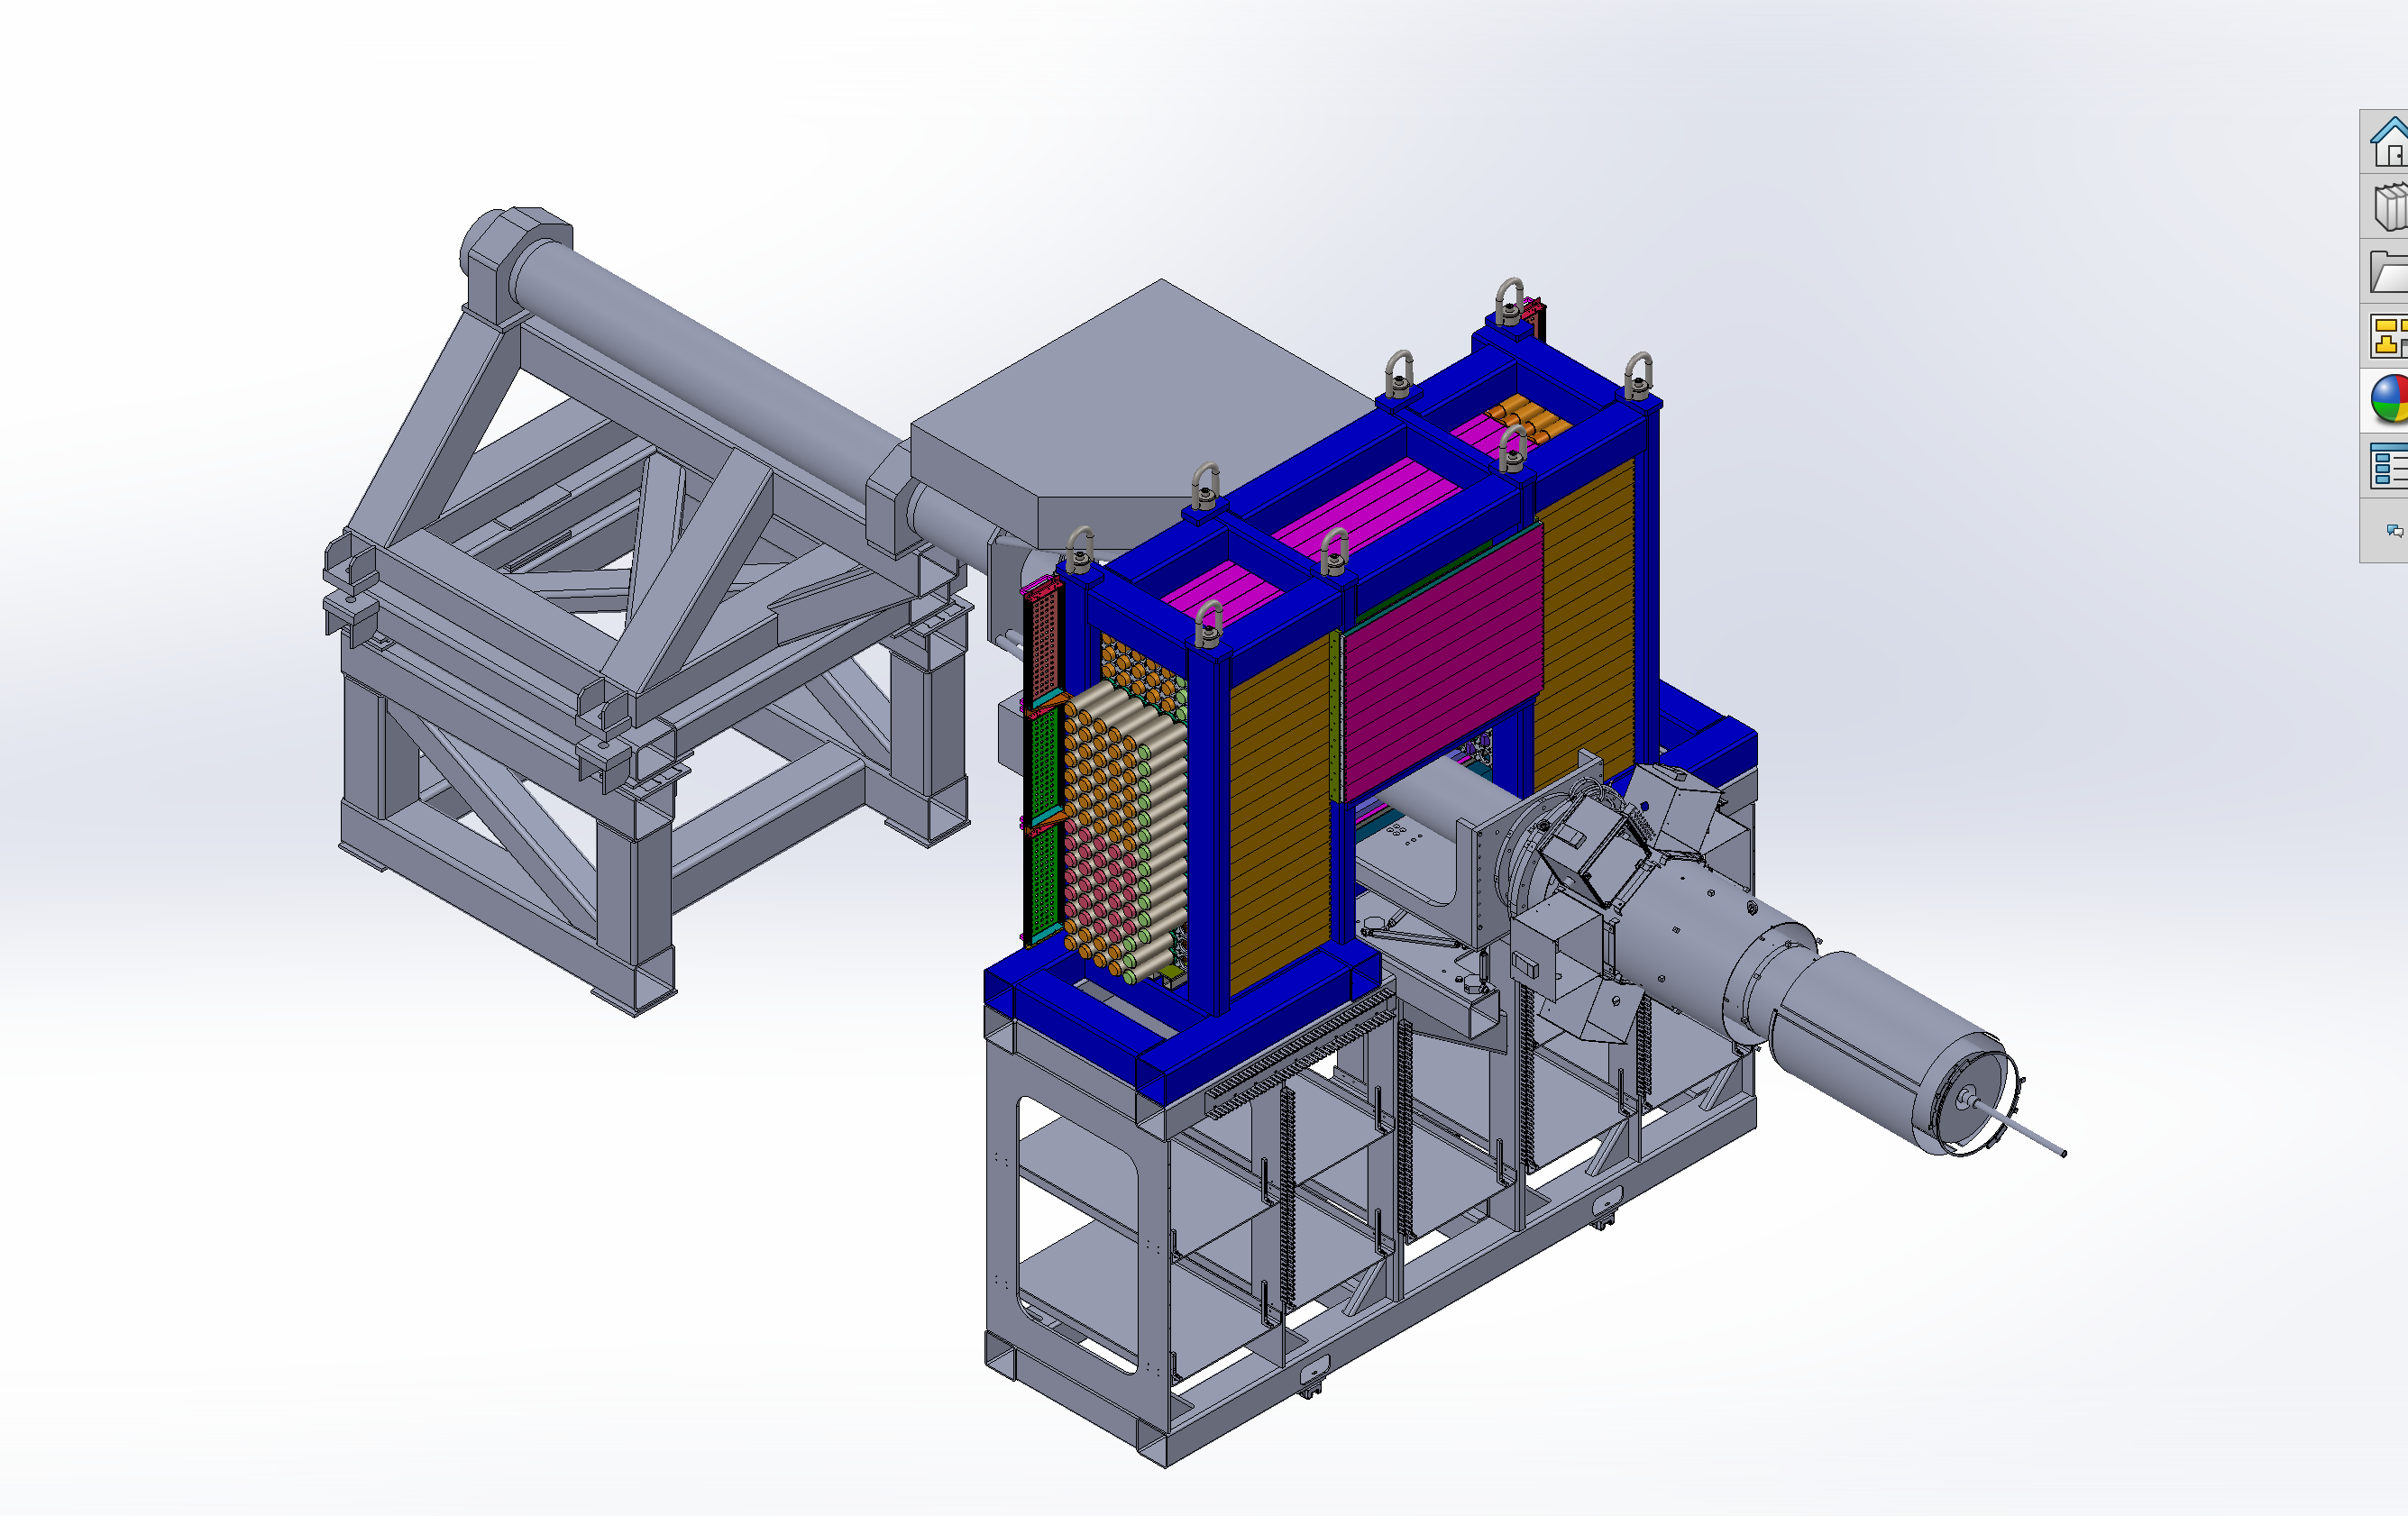
\includegraphics[width=0.48\textwidth]{BandInContext1.png}
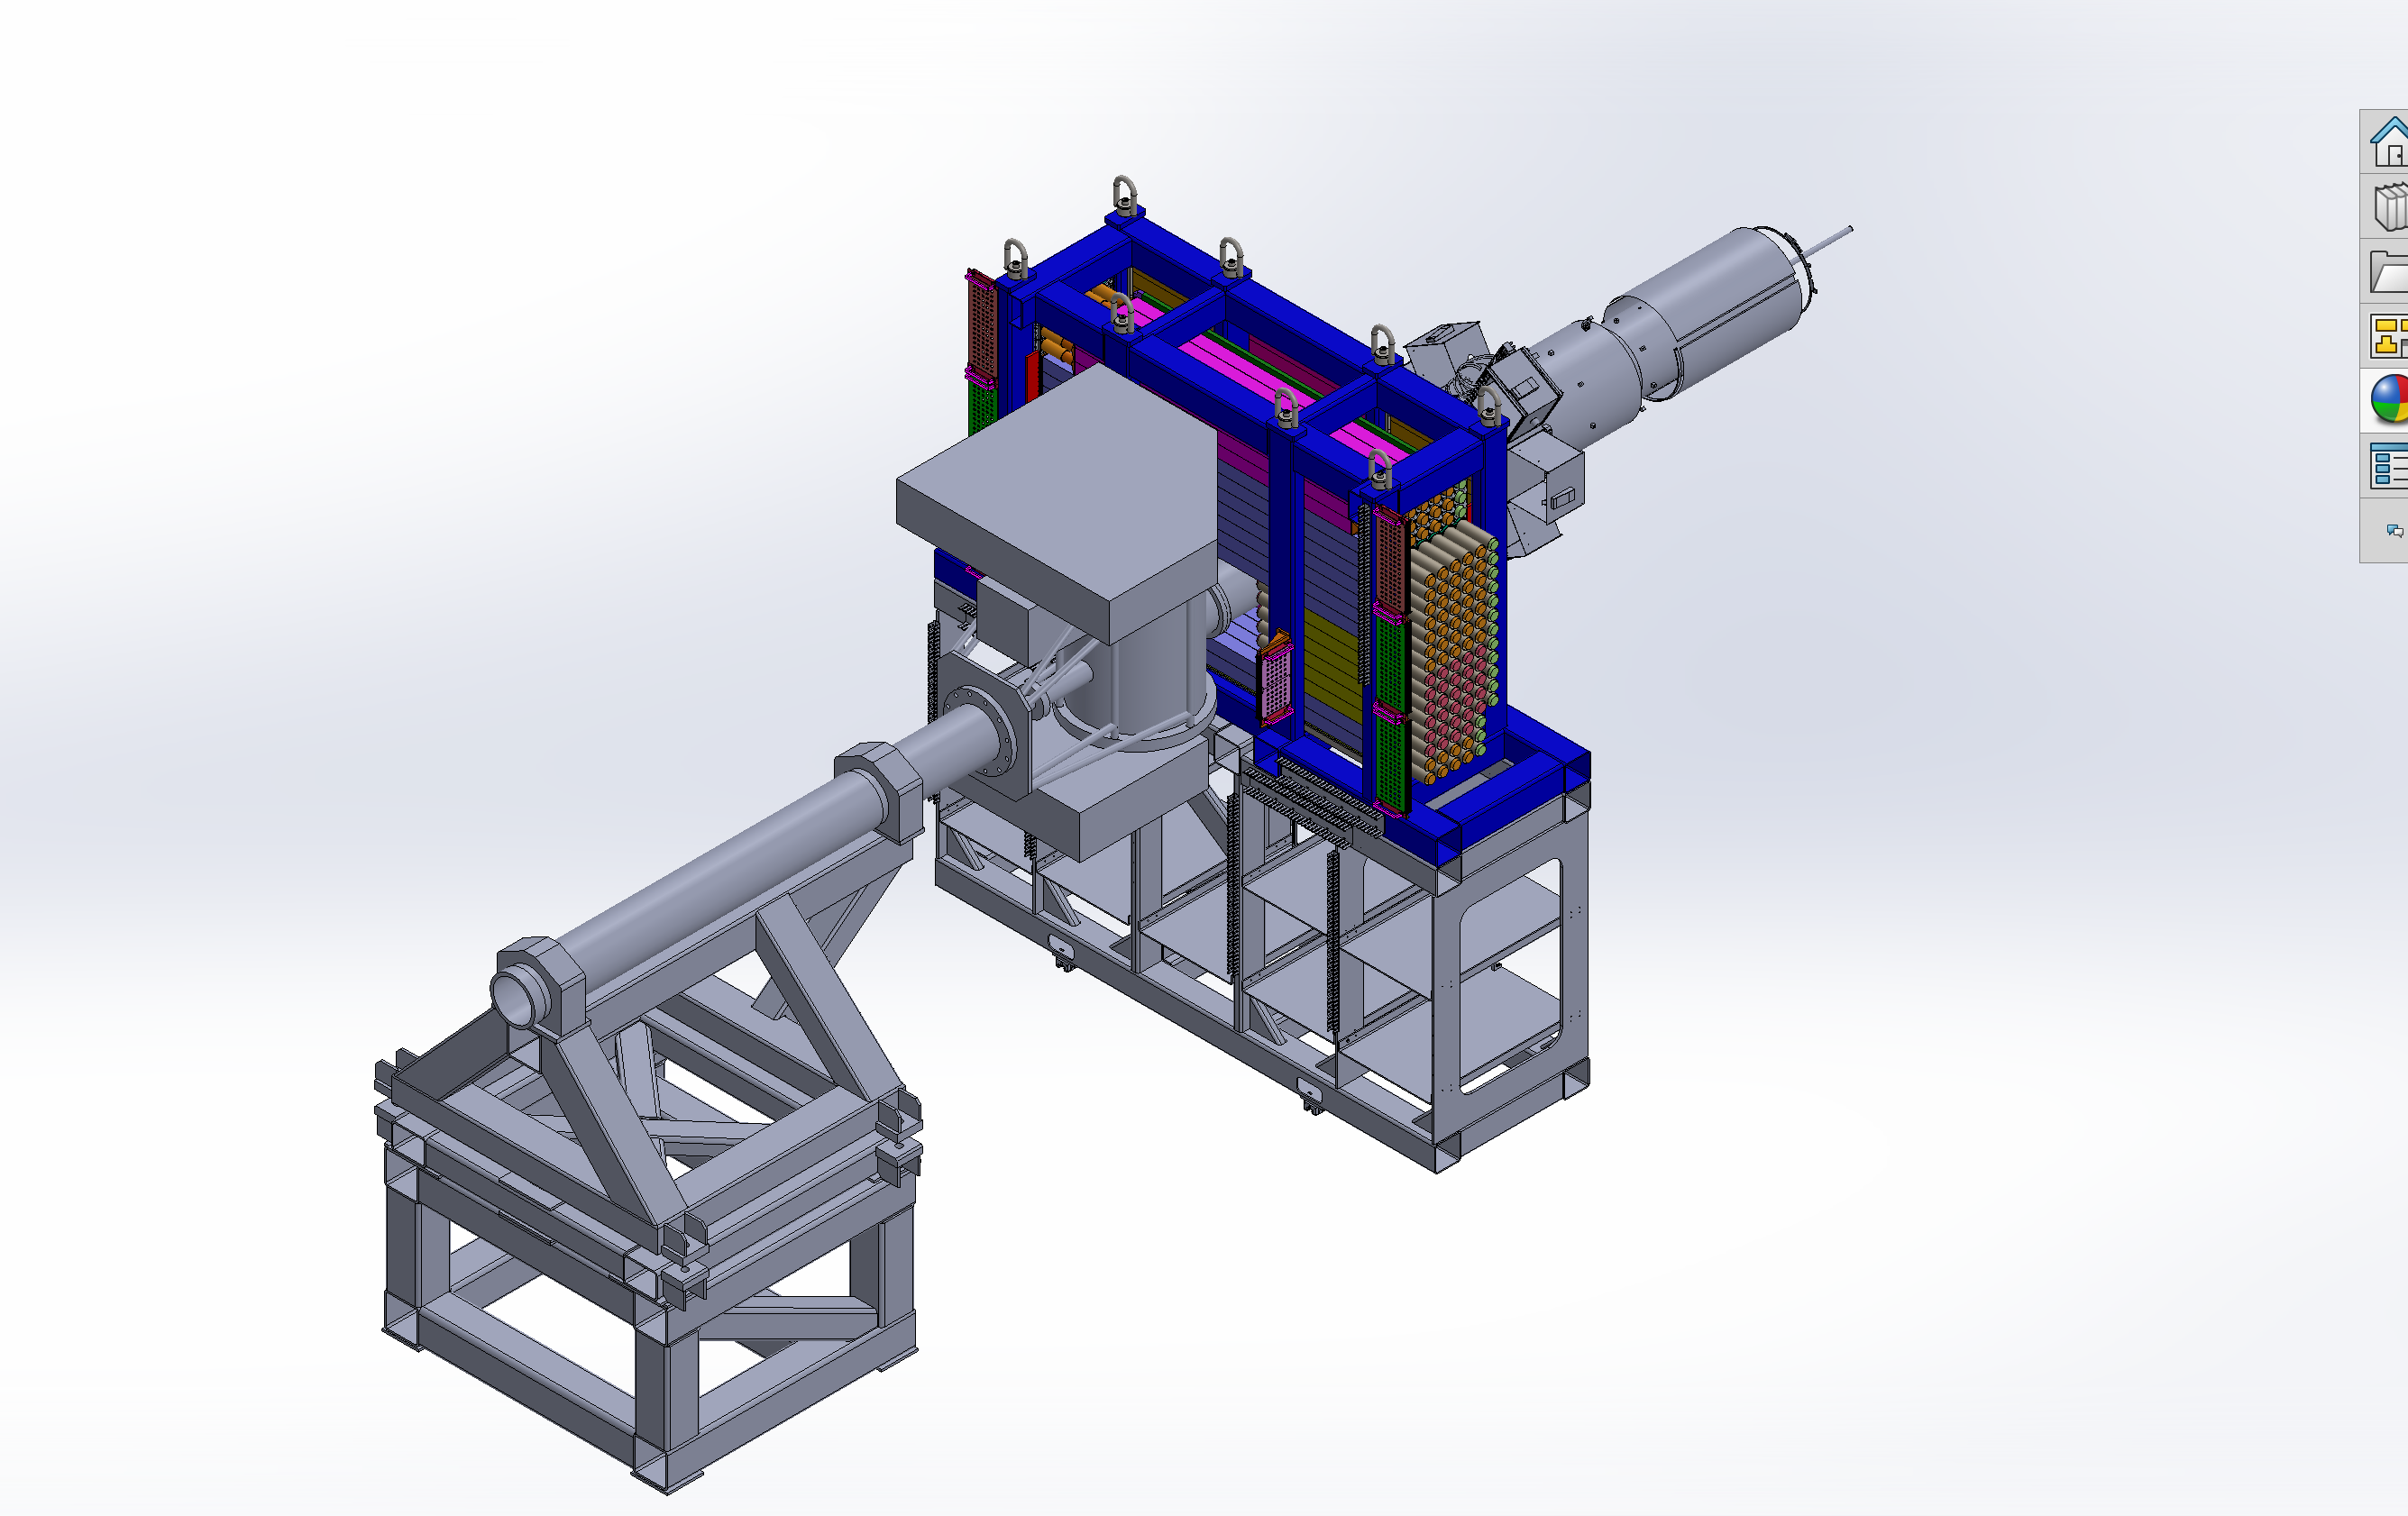
\includegraphics[width=0.48\textwidth]{BandInContext2.png}
 \caption{The BAND detector is shown with its surroundings: CLAS12 target, beam line and SVT cart. (Left) Beam is coming from top left. (Right) Beam is coming from bottom left. }
  \label{fig:bandcontext}
\end{figure}
The Backward Angle Neutron Detector (BAND) is placed at the top of the SVT cart upstream of the CLAS12 target. The detector in context of its surroundings (target, beam line and cart) is shown in Fig. \ref{fig:bandcontext}.
 
The active detector area consists of 116 scintillator bars, arranged in 5 layers with 18 vertically stacked bars. The arrangement of the bars is shown in Fig.~\ref{fig:design}. The bottom rows are only arranged in four layers due to obstruction from surrounding frames.

\begin{figure}[tb]
	\centering
			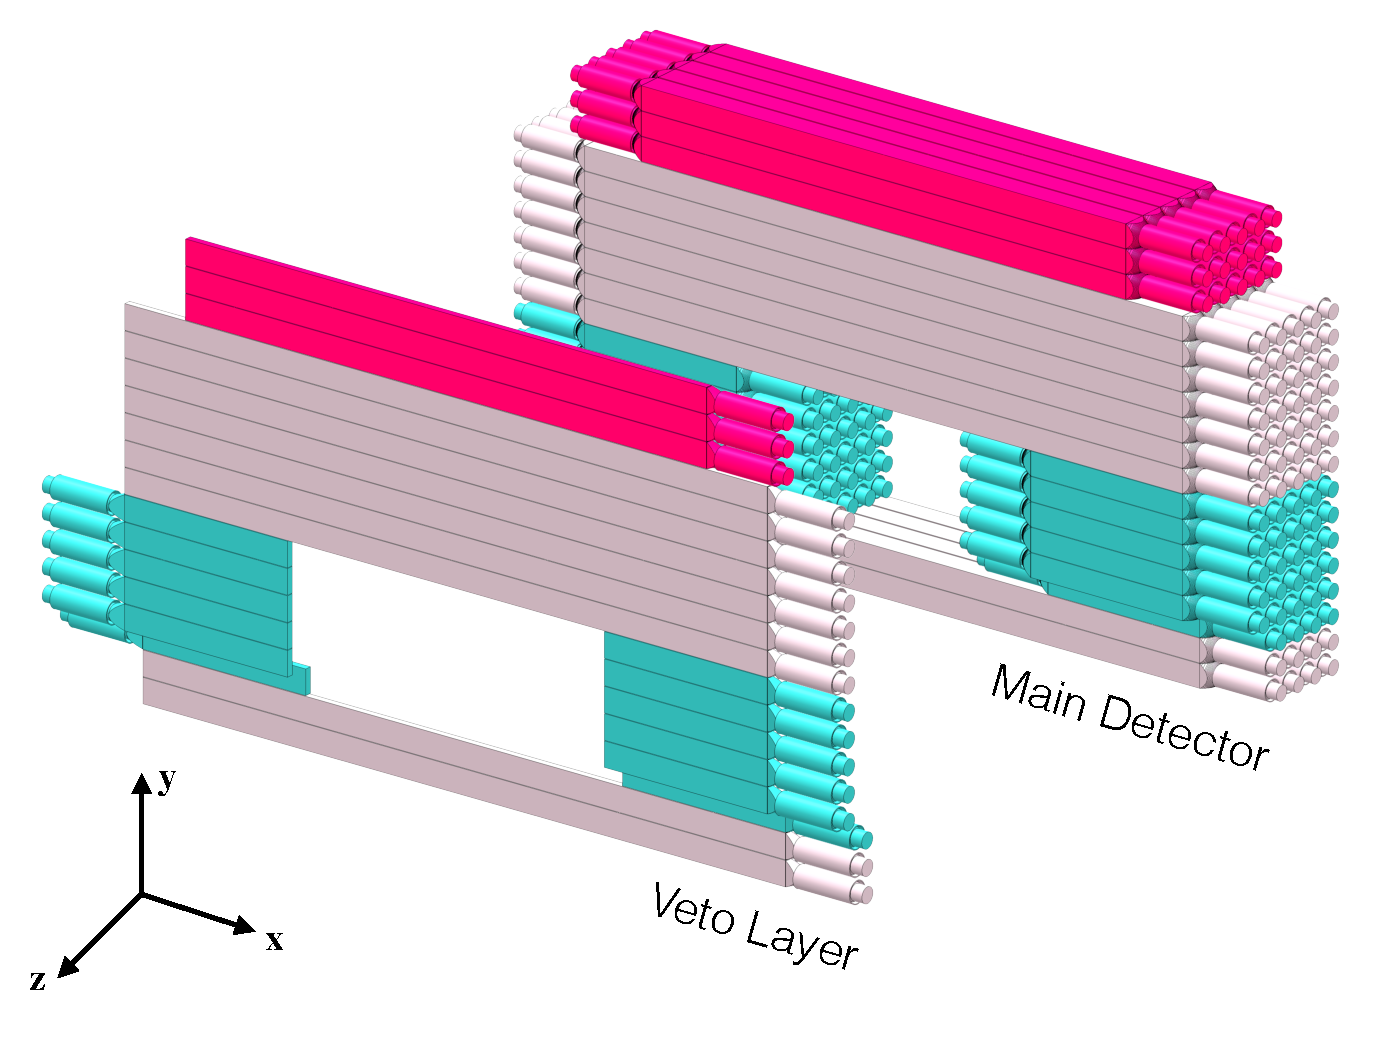
\includegraphics[width=0.48\textwidth]{band-schematic.pdf}
            \caption{BAND design of bars in the main
                   detector and the veto layer. The 164~cm long bars are shown in
                          red, the 202~cm bars in white
                          and the short, 51~cm bars in cyan. The position of
                          the PMTs for each bar is also shown. The beam direction corresponds to the $z$-axis.   }
		\label{fig:design}
\end{figure}

Each bar has a cross section of $7.2 \times 7.2\,\mathrm{cm}^{2}$ and are made of Bicron BC-408 scintillant. Three different long bars are used in the detector: 15 bars with a length of $164\,\mathrm{cm}$ (red in Fig.~\ref{fig:design}), 43 bars with a length of $202\,\mathrm{cm}$ (white in Fig.~\ref{fig:design}) and 58 short bars with a length of $51\,\mathrm{cm}$ (cyan in Fig.~\ref{fig:design}). The short bars are necessary for hole for the beam line and target installation. The total thickness is $36\,\mathrm{cm}$ giving a neutron detection efficiency of about 30\%.

All bars are read-out on both sides by PMTs (100 Hamamatsu R7724 and 132 ET 9214) giving a total of 232 active channels. Since the PMTs are placed in the fringe field region of the solenoid, and they are encased in a cylindrical shielding made up by a 2-mm-thick layer of mu-metal.

In front of the first active layer of BAND, a veto layer is installed with 24 scintillators bars which are read-out only on one side by Thorne EMI 9954KB PMTs. The bars have a cross section of $2 \times 7.2\,\mathrm{cm}^{2}$. The bars in the veto layer have the same length as the bars of one layer of the active detector area. The veto layer is also shown in Fig.~\ref{fig:design}.

The total number of channels for BAND including the veto layer is 256. Between BAND and CLAS a $2\,\mathrm{cm}$ lead shield is installed.
Next to the PMTs attached to the frame a patch panel is installed for the HV cables, signal cables and optical fibers from the laser calibration system.

\subsection{Read-out Electronics}
%TO BE INCLUDED
%PICTURE OF HV CRATES
%PICTURE OF SPLITTERS, DISCRIMINATORS, VME AND VXS CRATE WITH FADC and TDC.
%Detailed channel maps

\begin{figure}[tb]
	\centering
	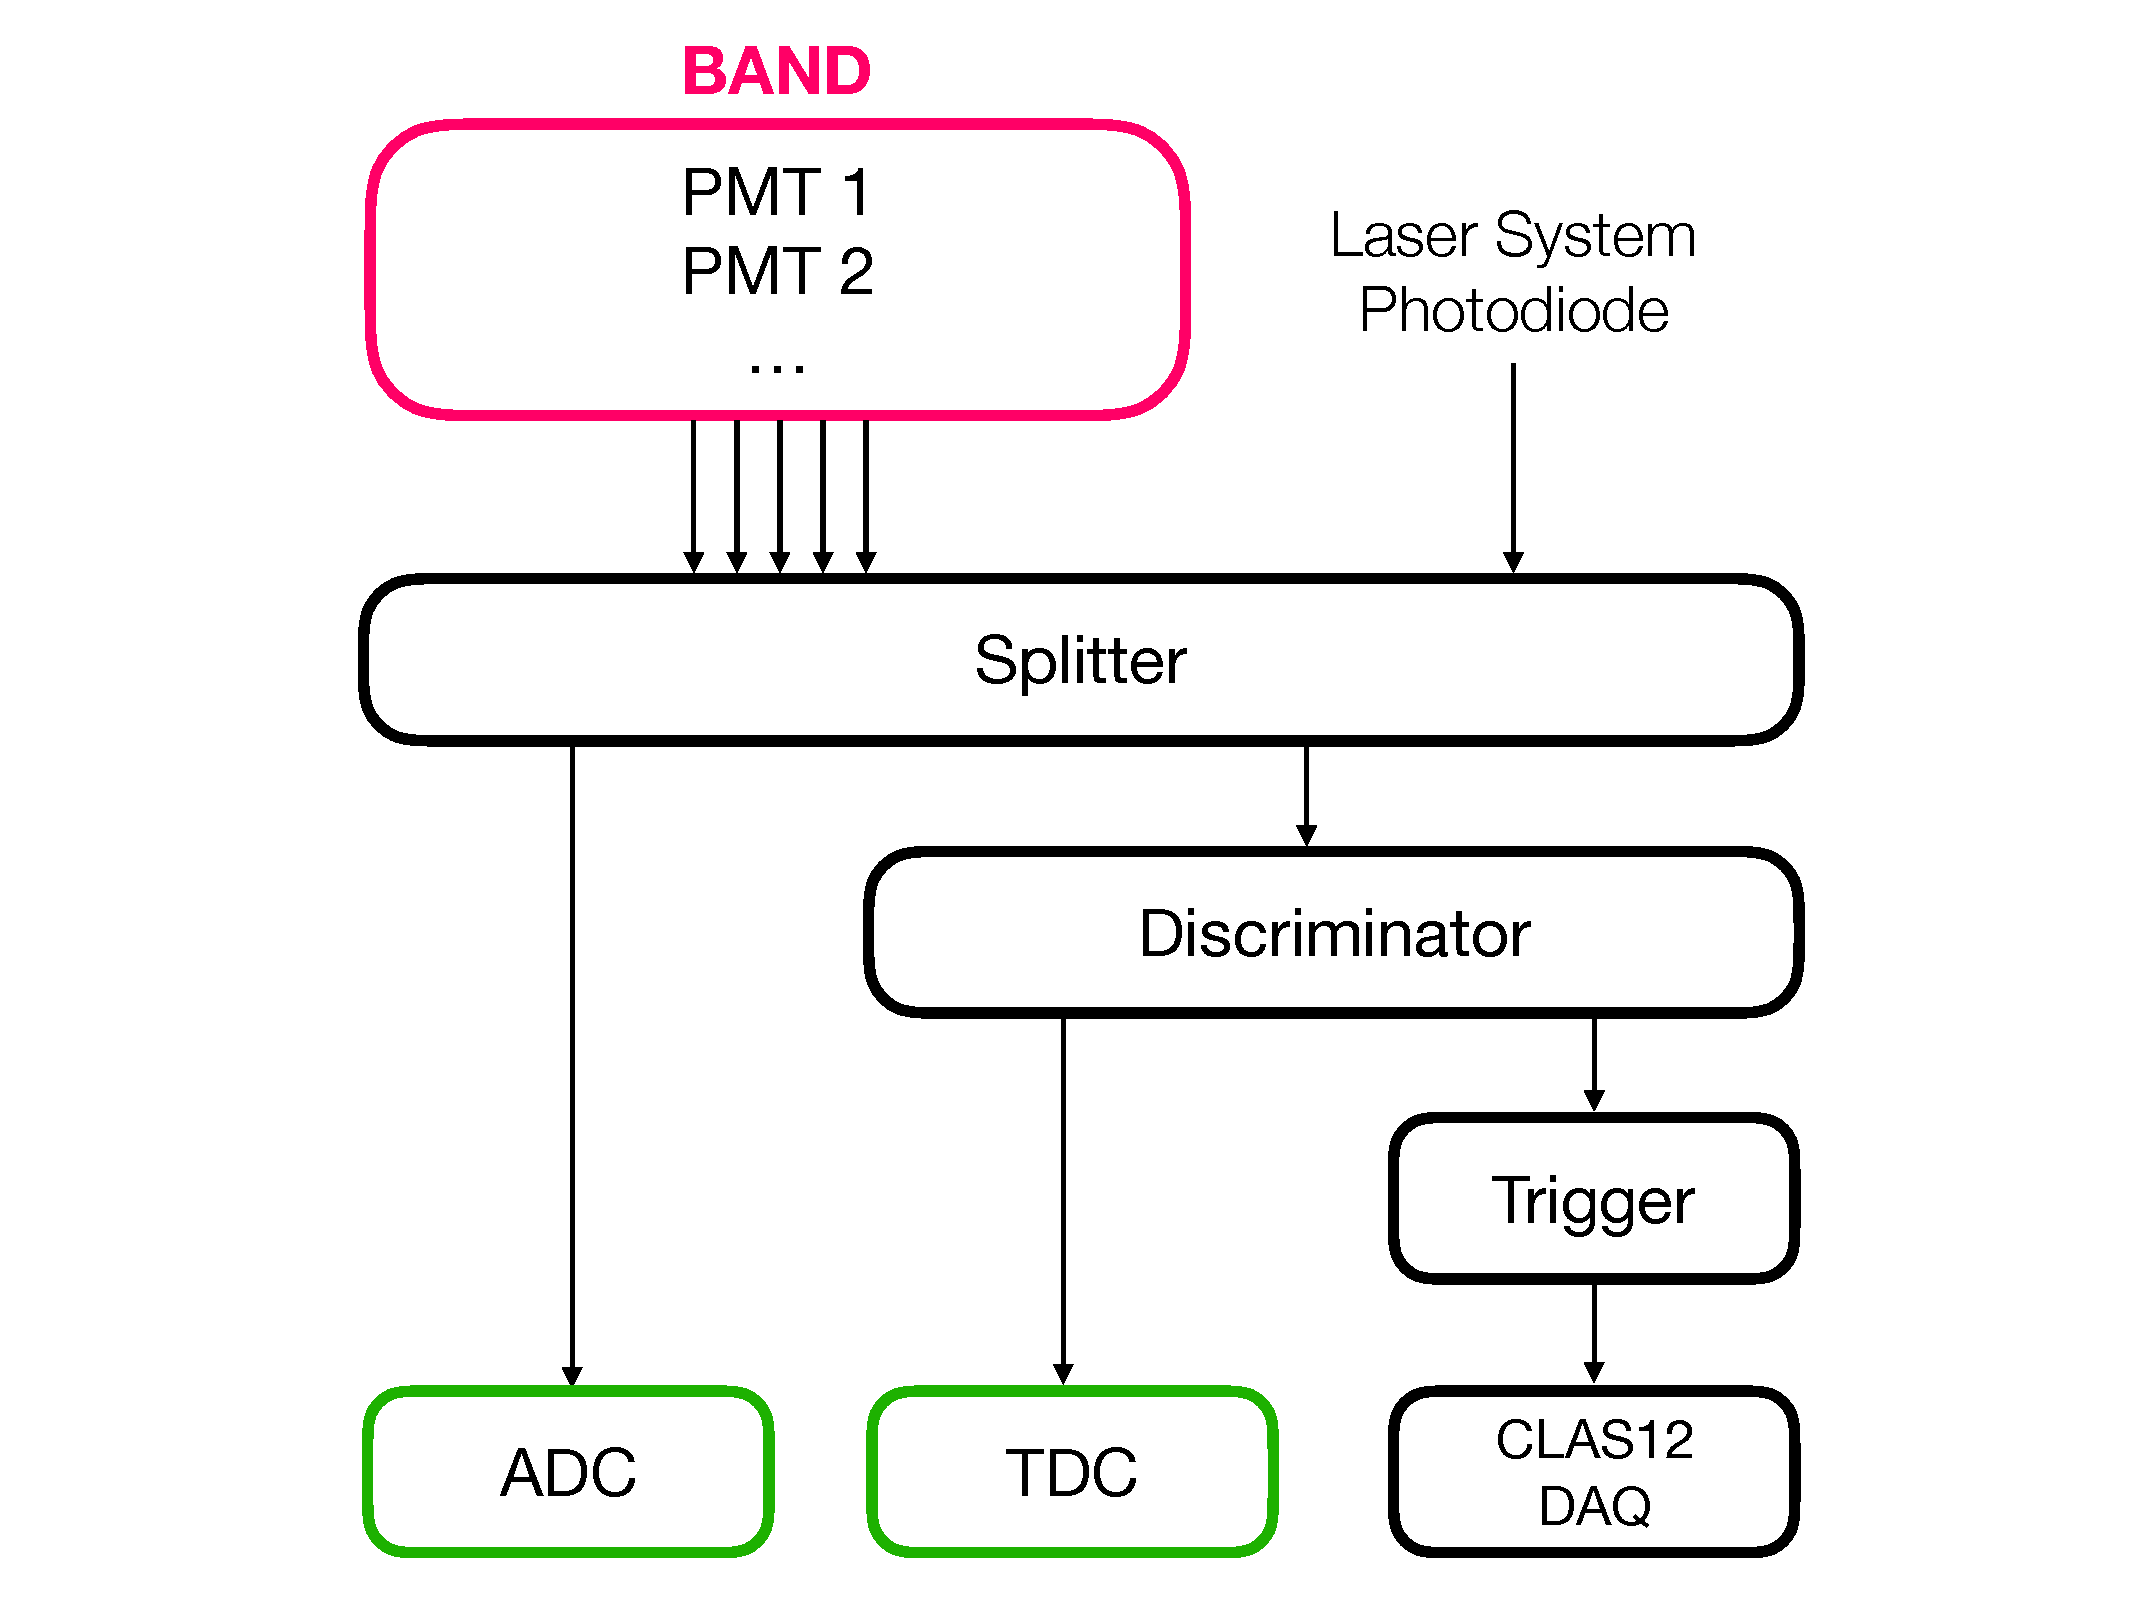
\includegraphics[width=0.58\textwidth]{electronics-diag.pdf}
	\caption{Electronic schematic of the BAND read-out. Every PMT signal is split and ADC and TDC information are obtained. Additional outputs of the discriminators are used to create single bar and cosmic-laser triggers from BAND.}
	\label{fig:electronic-diag}
\end{figure}

The high voltages for each PMT are provided by a multi-channel CAEN SYS4527 mainframe with eleven A1535SN cards with 24 channel each.
The HV are typically in the range of 1500 V.

A schematic drawing of the read-out electronics and its components is
shown in Fig.~\ref{fig:electronic-diag}. The signal of each PMT is
split to an ADC and TDC, read out independently.  The signal splitters
are custom made and have been used in previous experiments at
Jefferson Lab.  From the splitter one signal is sent to a 250-MHz sampling flash-ADCs (FADC) while the
other signal is sent to discriminators.  The discriminated time signal
goes to a TDC (CAEN VX1190A) with 100-ps resolution
per channel.

In total, the system consists of 16 flash-ADCs in one VXS crate, 16
discriminators and two TDCs in a VME crate and 16 splitters.
A trigger signal distribution card for the flash-ADCs and
trigger interface boards are installed in the crates. All components
are part of the standard CLAS12 electronics.

The detector is read out either by a trigger from the main CLAS12
trigger system or by stand-alone BAND 
triggers. The stand-alone triggers are used for tests and calibrations with cosmic rays, radioactive sources and the laser system. 
They are implemented by a programmable CAEN V1495 logic board. Such triggers include
a single bar trigger for source measurements and a
coincidence bar trigger for cosmics and laser measurements. The
coincidence trigger is also fed to the central CLAS12 trigger system
to allow monitoring of the detector by recording laser data during
experimental data taking. This laser-monitoring trigger rate is usually about 10
Hz, compared to the roughly $15-20\,\mathrm{kHz}$ trigger
rate from electron interactions in the target.




\subsection{Laser Calibration System}
%MISSING PICTURE
A UV laser system to calibrate BAND and monitor its
performance has been installed. 
The design and performance of the system is fully 
described in a NIM paper (Denniston et al., NIM A 973 (2020), 164177). 
The main component of the system is a picosecond pulsed diode laser 
(Teem Photonics STV-01E-140) with a wavelength 
of 355 nm. The laser can be triggered externally between 
$10-4000$ Hz. The light is only transported within fibers. Further components of the system are a mode scrambler, a 90:10 splitter whose outputs are connected to a reference photodiode (10\% output) and a variable optic attenuator (90\% output). The attenuator allows to vary the pulse intensity sent to the detector. It is connected to a custom SQS Vl\'aknov\'a Optika 1$\times$400 splitter which distributes the light to every bar of BAND. 

Each bar has an optical fiber glued to its center with UV-curable glue. We used an exposed fiber for the fiber-scintillant connection since it was a stable, reliable and easy option. The other end of the fiber is connected to the splitter through a patch panel attached to the BAND frame. 

The photodiode provides reference time for the laser system. The output
signal of the photodiode is inverted and shaped before it is sent to
the BAND read-out system. The photodiode signal is then digitized by the same ADCs and
TDCs which are used for the PMT signals.



\section{Information for Shift Workers}

\subsection{Shift Worker Responsibilities}
The shift worker in the Hall B Counting House has five responsibilities with regard to the BAND system:
\begin{enumerate}
\item Updating the Hall B electronic logbook with records of problems or system conditions (see Section~\ref{sssec:logbook}).
\item Contacting BAND system on-call personnel for any problems that are discovered (see Section~\ref{sssec:personel}).
\item Responding to BAND system alarms from the Hall B alarm handler (see Section~\ref{sssec:alarms}).
\item Turning on or off the high voltage (HV) for the BAND system using the HV control interface (see Section~\ref{ssec:hv}).
\item Monitoring the hit occupancy scalers for the system (see Section~\ref{ssec:guimonitoring}).
\end{enumerate}

\subsubsection{Updating the Logbook}
\label{sssec:logbook}
The electronic logbook (or e-log) is set up to run on a specified terminal in the Hall B Counting House. Shift workers are responsible for keeping an up-to-date and accurate record of any problems or issues concerning the BAND system. For any questions regarding the logbook, its usage, or on what is considered to be a “logbook worthy” entry, consult the assigned shift leader.
Note the shift worker should follow all posted or communicated instructions about entering BAND monitoring histograms or scaler information into the e-log. 
\subsubsection{Contacting the BAND System Personel}
\label{sssec:personel}
As a general rule, shift workers should spend no more than 10 to 15 minutes attempting to solve any problem that arises with the BAND system. At that point they should contact the assigned BAND on-call expert either to provide advice on how to proceed or to address the problem. \textcolor{red}{The BAND on-call phone number is (757)-310-7198.}

This document is divided into sections for shift workers and for BAND system experts. However, only BAND system experts (as listed in Section \ref{sec:experts}) are authorized to make changes to the BAND HV settings, to work on the hardware or electronics, or to modify the BAND crate settings. This division between shift worker responsibilities and expert responsibilities is essential to maintain in order to protect and safeguard the equipment, to ensure data collection is as efficient as possible, and to minimize down time. If the shift worker has any questions regarding how to proceed when an issue arises, the shift leader should be consulted.
\subsubsection{Hall B Alarm Handler}
\label{sssec:alarms}
The BEAST alarm handler system running in the Counting House monitors the entire Hall B Slow Controls system. This includes the HV and low voltage (LV) systems, gas systems, torus and solenoid controls, subsystem environment controls (e.g. temperature, humidity), and pulser calibration systems (among several others). The system runs on a dedicated terminal in the Counting House. One of the main responsibilities of the shift worker is to respond to alarms from this system, either by taking corrective action or by contacting the appropriate on-call personnel. %include reference Instructions and details on the alarm handler for Hall B are given in Ref. [2].

The only element of the BAND system monitored by the alarm handler is the HV system. Any time a channel trips off an alarm will sound. The alarm handler will identify the specific channel (or channels) that have tripped. These channels can be reset either through the alarm handler or through the nominal BAND HV control screens. These channels should be reset only after ensuring that whatever condition caused the trip (e.g. bad beam conditions) has been addressed.



\subsection{PMT High Voltage Controls}
\label{ssec:hv}
\subsection{HV control}
The BAND HV is controlled through the Hall B CSS suite which may be accessed from any PC in the Hall-B counting room, logging in as \textit{clasrun}. If it is not already running, it may be started by entering \textit{clascss} on a terminal. The BAND PMTs may be accessed by selecting \textbf{BAND} and then \textbf{BAND HV} from the subsystems in the main window, as shown in Fig. \ref{fig:CLASMenu}.

\begin{figure}
\centering
{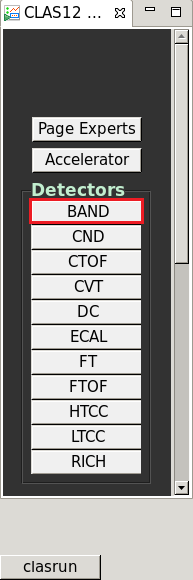
\includegraphics[width=.15\textwidth]{CLASMenuBAND.png}}
{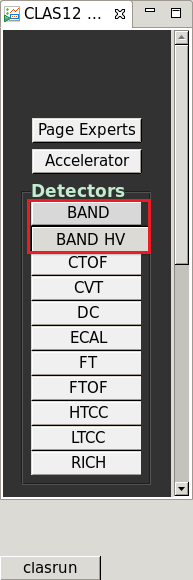
\includegraphics[width=.15\textwidth]{CLASMenuSubBAND.png}}

\caption{Location of BAND within CLAS12 slow-control main window.}
\label{fig:CLASMenu}
\end{figure}

\begin{figure}
\centering
{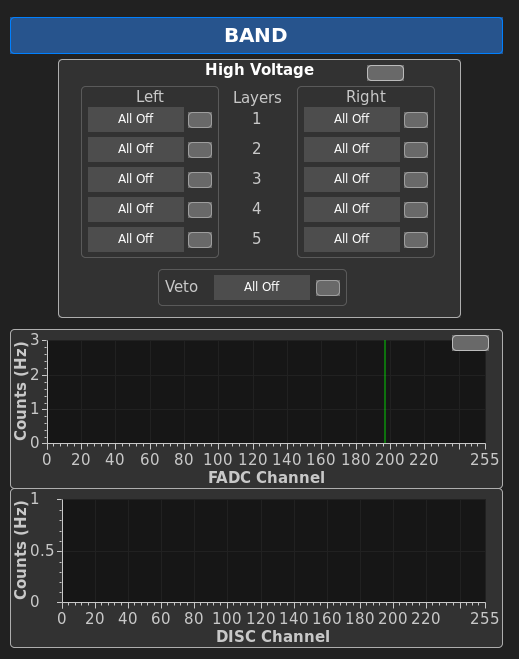
\includegraphics[width=.367\textwidth]{MainScreenshot.png}}
{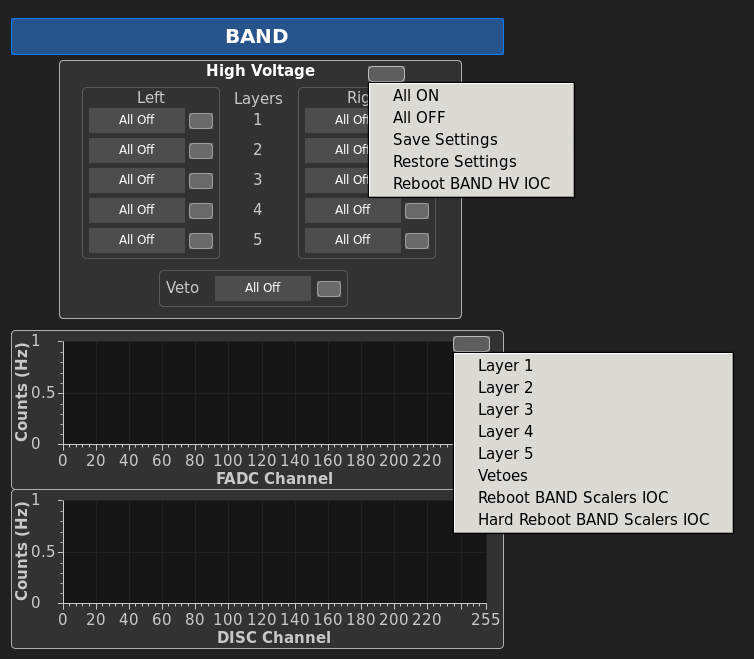
\includegraphics[width=.533\textwidth]{MainScreenshotTwoMenus.png}}

\caption{BAND main screen, including location of main and scaler menus.}
\label{fig:BANDMenu}
\end{figure}
Upon this selection, the BAND main screen will be displayed as in Fig. \ref{fig:BANDMenu} (left).
This interface allows for HV operations at a number of functionality levels:
\begin{itemize}
\item All channels of the BAND system
\item All channels on either the left or right side on every BAND bar per layer
\item All channels of the veto layer of BAND
\end{itemize}
The HV Control Interface screen also provides a color key to indicate the channel status:
\begin{itemize}
\item HV off - no highlight color (channel color dark green)
\item HV on - bright green
\item HV ramping up or ramping down - orange
\item HV trip - red
\item Communication problem - red
\item Undefined channel status - magenta
\end{itemize}
For the shift worker the most common operations are:
\begin{enumerate}
\item To turn the HV for all system PMTs on or off. This is accomplished by clicking the button in the upper right corner. This pops up a sub-menu with the relevant options “Turn All Off” and “Turn All On” (see Fig. \ref{fig:BANDMenu} (right)).
\item To turn individual PMTs on or off. This is accomplished by clicking on the button representing the layer (1-5) and side (L/R) or veto for the channel of interest. This brings up a submenu where the detailed HV screen for the layer can be choosen. %Include pic here for a layer 
In the next screen the channel HV can be toggled on and off by clicking on the button in the “Pw” (Power) column.
\item To turn the HV for all PMTs in a single layer and side or vetos on and off. This is accomplished by clicking on the button next to each layer and side. This pops up a sub-menu with the relevant options “Turn Layer XX Off” and “Turn Layer XX On”.
\end{enumerate}
.
%If the “Open Channel Controls” option shown in Fig. xx is selected, a “novice” window is opened as shown in Fig. xx. 
The window to control every PMT shows the monitored channel voltage and current ($V_{mon} (\mathrm{V})$ and $I_{mon} (\mathrm{\mu A}))$, the channel status (OFF, ON), and the set channel voltage and current ($V_{set} (\mathrm{V})$ and $I_{set} (\mathrm{\mu A}))$. If desired, shift workers can toggle the HV settings for single channels on or off through this interface.

In the upper left corner of this “Channel Controls” window is a button marked “expert” % that brings up the window shown in Fig. 11. 
This allows changes to the system settings for the maximum channel current, maximum channel voltage setting, and the channel HV ramp up and ramp down rates. Clicking on the “novice” button in the upper left corner toggles between the expert and novice screens. \textcolor{red}{The expert screen should only be used by the list of authorized BAND personnel given in Section \ref{sec:personnel}.}
\subsection{Resetting the IOCs}
If there is a controls problem indicated by the appearance of magenta channels or communication error in Fig. \ref{fig:BANDMenu}, which typically appears for all PMTs in a layer, the usual cause is an issue of communication between the IOC computer and the HV mainframe. To reboot the IOC for a given sector, click on the button in the upper right corner. This pops up a sub-menu with the relevant option "Reboot BAND HV IOC" (see Fig. \ref{fig:BANDMenu} (right)). The reboot will take less than two minutes to complete and the magenta or communication problem channel indicators should all disappear. If rebooting the IOC does not solve the problems, contact the Slow Controls system expert.

Note that the IOCs can be also rebooted through the “IOCs” button on the CSS control panel within the “Subsystems” portion of the interface. However, this should be usually done with the support of the system expert.

\section{Information for System Experts}
\label{sec:experts}
\subsection{Responsibilities}
The BAND system experts have several key responsibilities:
\begin{enumerate}
\item Complete hot checkout sign-off before the start of each run period %including cite to a subchapter
\item Respond to calls on the on-call phone to resolve issues with the BAND system during data taking %including cite to a subchapter
\item Take initial gain calibration runs with cosmics and adjust the system HV settings %including cite to a subchapter
\item Take laser calibration runs for timing calibrations for run times
\item Monitor the system performance periodically with the bandmon expert monitoring suite %including cite to a subchapter
\item Make repairs to the hardware during maintenance periods.
All issues found, work completed, or questions related to the BAND system should be entered into the e-log (HBLOG and HBBAND).
\end{enumerate}

\subsection{Initial Operation}
The initial operation of BAND after each prolonged downtime should be carried out by experts. 

To turn the detector on each of the electronic crates, and the HV crate must be powered and switched on. Each of the HV channels could be either turned on manually or remotely by means of the HV GUI. Switching on the channels remotely is the preferable method. 

The set values for the HV for the individual PMTs for the first operation are determined by cosmics measurements to equalize gain and possible measurements with sources afterwards.

The laser system will be powered and used calibration runs or monitoring during beam times.

\section{Slow Controls}

\subsection{Detector Monitoring}
\label{ssec:guimonitoring}
The monitoring software for BAND can be opened with the command 'bandmon' on a terminal on every clonpc machine. This will open the monitoring GUI based on similar GUIs for ECAL/PCAL developed by Cole Smith. 
%MISSING: more details about the controlling
\subsection{Laser Calibration System}

The laser system is controlled by the GUI shown in Fig. \ref{fig:LaserMenu}. The GUI may be accessed from any PC in the Hall-B counting room.
%MISSING: more details about the controlling.
\begin{figure}
\centering
{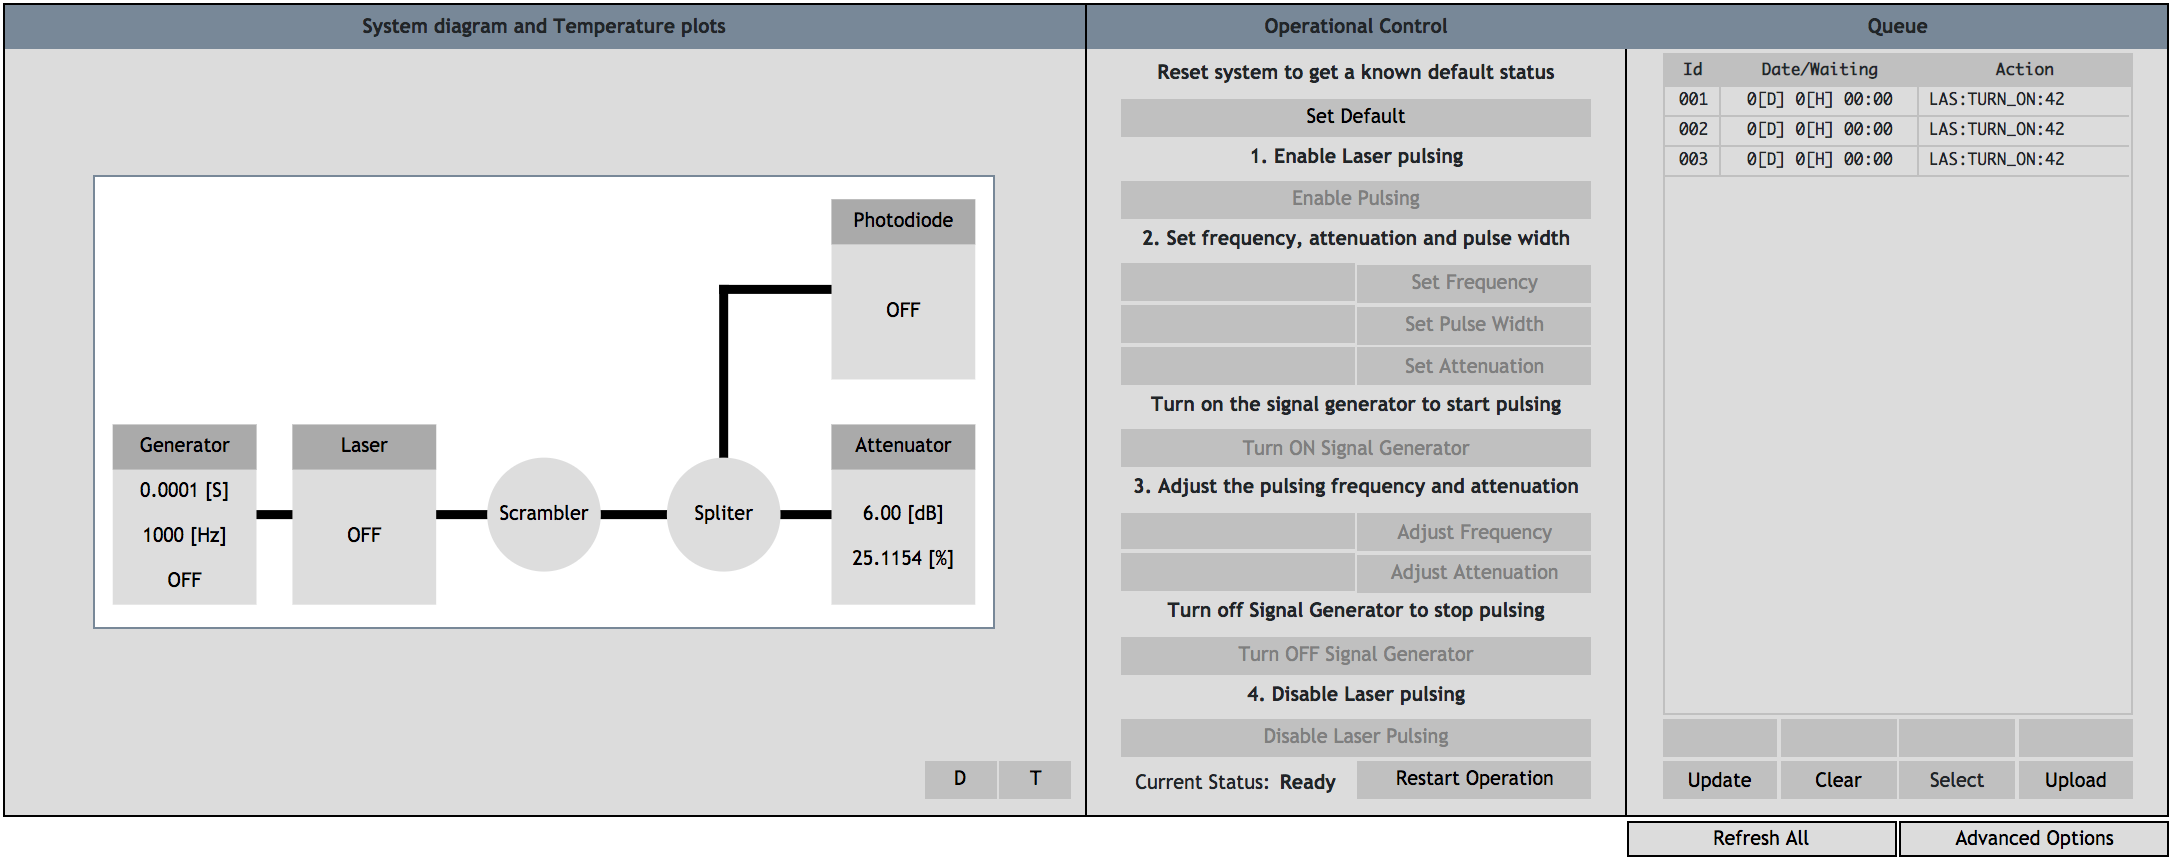
\includegraphics[width=.9\textwidth]{laserscreen_basic.png}}
{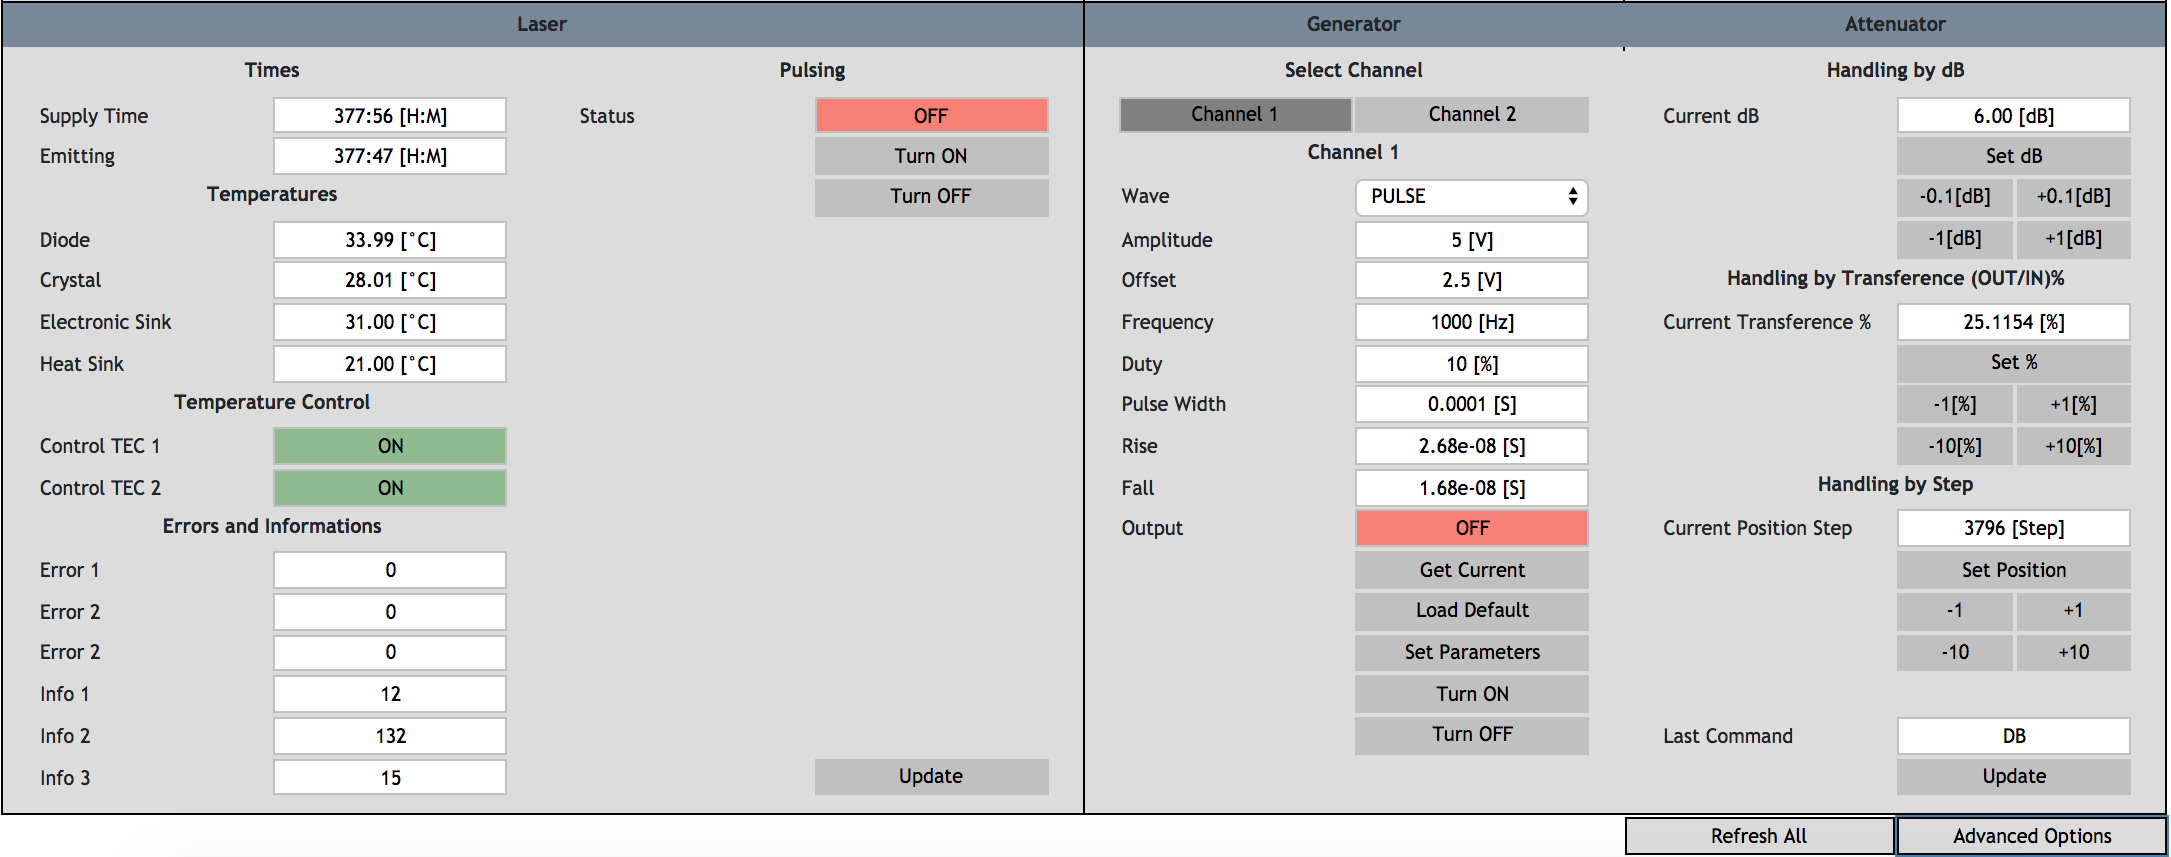
\includegraphics[width=.9\textwidth]{laserscreen_adv.png}}

\caption{Image of the GUI for the Laser Calibration System.}
\label{fig:LaserMenu}
\end{figure}

\section{Maintenance}
Given the location of BAND outside of the solenoid, most of BAND is accessible after installation. If needed PMTs on the outer ends of the scintillator bars could be replaced without moving other parts. However, the inner PMTs adjoint to the target and beam line of the shorter bars are not directly accessible. In this case BAND and the SVT cart needs to be pushed back upstream on the crane in position during installation.
Detailed plans for replacing PMTs are under development.

Exchanging cables for HV and signals can be easily done without moving BAND.

\section{Responsible Personnel}
\label{sec:personnel}
Individuals responsible for the system are:

\begin{table}[!htb]
 \centering
 \begin{tabular}{|c|c|c|c|c|}
\hline
 Name&Dept.&Phone&email&Comments \\ \hline
 Expert on call &  & (757)310-7198 & & 1st contact \\ \hline
Florian Hauenstein & JLab & & \href{mailto:hauenst@jlab.org}{\nolinkurl{hauenst@jlab.org}} & 2nd contact \\ \hline
O. Hen & MIT & &\href{mailto:hen@mit.org}{\nolinkurl{hen@mit.org}}& 3rd contact \\ \hline
L. Weinstein & ODU &  &\href{mailto:weinstein@jlab.org}{\nolinkurl{weinstein@jlab.org}}& 4rd  contact  \\ \hline

\end{tabular}
\caption{Personnel responsible for the Backward Angle Neutron Detector.} 
\label{table:personnelband}
\end{table}

%Personnel for the different subsystems. Laser system, Electronics extra.

\begin{table}[!htb]
 \centering
 \begin{tabular}{|c|c|c|c|c|}
\hline
 Name&Dept.& email&Comments \\ \hline
Florian Hauenstein & JLab &  \href{mailto:hauenst@jlab.org}{\nolinkurl{hauenst@jlab.org}} & Staff \\ \hline
Sara Ratliff & GWU & \href{mailto:ratliff_sara@gwmail.gwu.edu}{\nolinkurl{ratliff_sara@gwmail.gwu.edu}}& PhD \\ \hline
Caleb Fogler & ODU &  \href{mailto:cfogler@jlab.org}{\nolinkurl{cfogler@jlab.org}}& PhD  \\ \hline
Andrew Denniston & MIT &  \href{mailto:awild@jlab.org}{\nolinkurl{awild@jlab.org}}& PhD \\ \hline

\end{tabular}
\caption{List of trained BAND system experts.} 
\label{table:expertsband}
\end{table}

\end{document}
